
\newlength{\PageHeight}
\newlength{\PageWidth}
% ==============================================
% 一、基础框架 & 页面布局
% ==============================================
%\documentclass[17pt]{beamer}
%\setlength{\PageHeight}{13.5cm}
%\setlength{\PageWidth}{24cm} 

\documentclass[20pt]{beamer}
\setlength{\PageHeight}{19.05cm}
\setlength{\PageWidth}{33.866cm} 

% 设置页面边距变量为长度寄存器
\newlength{\PageLeft}
\newlength{\PageRight}
\newlength{\PageTop}
\newlength{\PageBottom}

\setlength{\PageLeft}{0.10498\PageHeight}
\setlength{\PageRight}{0.10498\PageHeight} 
\setlength{\PageTop}{0.07874\PageHeight} 
\setlength{\PageBottom}{0.10498\PageHeight}

% 自定义宽屏尺寸
\usepackage{geometry}
\geometry{
    paperwidth=\PageWidth,
    paperheight=\PageHeight,
    left=\PageLeft, right=\PageRight,
    top=\PageTop, bottom=\PageBottom
}

% 关闭默认导航、侧边栏、页眉
\setbeamertemplate{navigation symbols}{}
\setbeamertemplate{headline}{}
\setbeamertemplate{sidebar left}{}
\setbeamertemplate{sidebar right}{}

% 全局背景
\pagecolor{white}

% ==============================================
% 二、宏包加载（按依赖顺序）
% ==============================================
% 中日英字体 & 数学字体（XeLaTeX 专用顺序）
\usepackage{fontspec}
\usepackage{xeCJK}
\xeCJKsetup{CJKmath=true} % 支持公式内中文
\usepackage{unicode-math}

% 图形、颜色、绘图
\usepackage{graphicx}
\usepackage{xcolor}
\usepackage{tikz}
\usetikzlibrary{positioning}
\usetikzlibrary{backgrounds}
\usepackage{float}

% 表格
\usepackage{booktabs, multirow, bigstrut}

% 数学环境
\usepackage{amsfonts, amsmath, amsthm}
\usepackage{amssymb,bm,mathrsfs} % 数学符号支持


% 算法
\usepackage{algorithm, algpseudocode}

% 代码高亮
\usepackage{listings}

% 图表子图 & 标题
\usepackage{caption, subcaption}

% 多栏排版
\usepackage{multicol}

% ==============================================
% 三、全局段落格式
% ==============================================
\linespread{1.3}                 % 行距
\setlength{\parindent}{2em}      % 首行缩进
\BeforeBeginEnvironment{minipage}{\noindent}
\setlength{\parskip}{0.5\baselineskip}  % 段后0.5行
% ==============================================
% 四、字体配置（思源系列 + 英文字体）
% ==============================================
% 中文无衬线字体（思源黑体）
\setCJKsansfont[
    Path              = ./font/,
    Extension         = .otf,
    UprightFont       = SourceHanSansCN-Regular,
    BoldFont          = SourceHanSansCN-Bold,
    ItalicFont        = SourceHanSansCN-Regular,
    BoldItalicFont    = SourceHanSansCN-Bold,
    AutoFakeBold      = false,
    ItalicFeatures    = {FakeSlant = 0.15},
    BoldItalicFeatures= {FakeSlant = 0.15},
    Mapping           = fullwidth-stop% 把中文句号自动转化英文小圆点
]{}
% \setCJKsansfont{Microsoft YaHei} % 也可替换为微软雅黑（但需注意版权问题）

% 中文衬线字体（思源宋体）
\setCJKmainfont[
    Path              = ./font/,
    Extension         = .otf,
    UprightFont       = SourceHanSerifCN-Regular,
    BoldFont          = SourceHanSerifCN-Bold,
    ItalicFont        = SourceHanSerifCN-Regular,
    BoldItalicFont    = SourceHanSerifCN-Bold,
    AutoFakeBold      = false,
    ItalicFeatures    = {FakeSlant = 0.15},
    BoldItalicFeatures= {FakeSlant = 0.15},
    Mapping           = fullwidth-stop% 把中文句号自动转化英文小圆点
]{}
%\setCJKmainfont{SimSun} % 也可替换为宋体（但需注意版权问题）

% 中文等宽字体（霞鹜文楷）
\setCJKmonofont[
    Path              = ./font/,
    Extension         = .ttf,
    UprightFont       = LXGWWenKaiMono-Regular,
    BoldFont          = LXGWWenKaiMono-Medium,
    ItalicFont        = LXGWWenKaiMono-Regular,
    BoldItalicFont    = LXGWWenKaiMono-Medium,
    AutoFakeBold      = false,
    ItalicFeatures    = {FakeSlant = 0.15},
    BoldItalicFeatures= {FakeSlant = 0.15},
    Mapping           = fullwidth-stop% 把中文句号自动转化英文小圆点
]{}
%\setCJKmonofont{KaiTi} % 也可替换为楷体（但需注意版权问题）

% 英文字体
\setmainfont{TeX Gyre Termes}
\setsansfont{TeX Gyre Heros}
\setmathfont{TeX Gyre Termes Math} % 或选择 Latin Modern Math
\setmonofont[
    Path              = ./font/,
    Extension         = .otf,
    UprightFont       = SourceCodePro-Regular,
    BoldFont          = SourceCodePro-Bold,
    ItalicFont        = SourceCodePro-It,
    BoldItalicFont    = SourceCodePro-BoldIt,
    AutoFakeBold      = false
]{}
%\setmonofont{TeX Gyre Cursor} %等宽也可以替换成这个字体


% ==============================================
% 五、全局色彩定义
% ==============================================
\definecolor{NPUBlue}{RGB}{0,78,162}
\definecolor{NPUDarkBlue}{RGB}{0,51,102}
\definecolor{ExampleGreen}{RGB}{0,128,64}
\definecolor{AlertOrange}{RGB}{204,102,0}
\definecolor{LightTea}{RGB}{245,241,236}

% ==============================================
% 六、Beamer 全局颜色样式
% ==============================================
% 列表符号颜色
\setbeamercolor{item}{fg=NPUBlue}
\setbeamercolor{subitem}{fg=NPUBlue}
\setbeamercolor{subsubitem}{fg=NPUBlue}
\setbeamercolor{enumerate item}{fg=NPUBlue}

% 各级标题颜色
\setbeamercolor{frametitle}{fg=NPUBlue}
\setbeamercolor{framesubtitle}{fg=NPUBlue}
\setbeamercolor{section title}{fg=NPUBlue}
\setbeamercolor{subsection title}{fg=NPUBlue}

% 线条、脚注、标签
\setbeamercolor{separation line}{fg=NPUBlue}
\setbeamercolor{footnote}{fg=NPUBlue}
\setbeamercolor{label}{fg=NPUBlue}

% 图表标题汉化 + 颜色
\renewcommand{\figurename}{图：}
\renewcommand{\tablename}{表：}
\captionsetup{labelfont = {color=NPUBlue}, labelsep=space}

% 参考文献样式与颜色
\setbeamertemplate{bibliography item}[text]
\setbeamercolor{bibliography item}{fg=NPUBlue}
\setbeamercolor{bibliography entry author}{fg=NPUBlue}
\setbeamercolor{bibliography entry title}{fg=black}
\setbeamercolor{bibliography entry location}{fg=NPUBlue!60}

% ==============================================
% 七、区块环境（块、定理、定义、示例、警示等）
% ==============================================
% 基础区块外观：圆角、无阴影、标题加粗
\setbeamertemplate{blocks}[rounded][shadow=false]
\setbeamerfont{block title}{series=\bfseries}

% 基础区块配色
\setbeamercolor{block title}{fg=white, bg=NPUBlue}
\setbeamercolor{block body}{fg=black, bg=NPUBlue!10}

% 示例区块（绿色）
\renewenvironment{exampleblock}[1]
{%
  \setbeamercolor{block title}{fg=white, bg=ExampleGreen}
  \setbeamercolor{block body}{fg=black, bg=ExampleGreen!10}
  \begin{block}{#1}
}
{\end{block}}

% 警示区块（橙色）
\renewenvironment{alertblock}[1]
{%
  \setbeamercolor{block title}{fg=white, bg=AlertOrange}
  \setbeamercolor{block body}{fg=black, bg=AlertOrange!10}
  \begin{block}{#1}
}
{\end{block}}

% 定理、引理、推论、命题
\renewenvironment{theorem}[1][]{\begin{block}{定理\ifx\relax#1\relax\else：#1\fi}}{\end{block}}
\renewenvironment{lemma}[1][]{\begin{block}{引理\ifx\relax#1\relax\else：#1\fi}}{\end{block}}
\renewenvironment{corollary}[1][]{\begin{block}{推论\ifx\relax#1\relax\else：#1\fi}}{\end{block}}
\newenvironment{proposition}[1][]{\begin{block}{命题\ifx\relax#1\relax\else：#1\fi}}{\end{block}}

% 定义（青色系）
\renewenvironment{definition}[1][]{
    \setbeamercolor{block title}{bg=cyan!70!black, fg=white}
    \setbeamercolor{block body}{bg=cyan!5}
    \begin{block}{定义\ifx\relax#1\relax\else：#1\fi}}{\end{block}}

% 例子
\renewenvironment{example}[1][]{\begin{exampleblock}{例子\ifx\relax#1\relax\else：#1\fi}}{\end{exampleblock}}

% 习题（紫色系）
\newenvironment{exercise}[1][]{
    \setbeamercolor{block title}{bg=purple!70!black, fg=white}
    \setbeamercolor{block body}{bg=purple!5}
    \begin{block}{习题\ifx\relax#1\relax\else：#1\fi}}{\end{block}}

% 注记（复用警示块）
\newenvironment{remark}[1][]{\begin{alertblock}{注记\ifx\relax#1\relax\else：#1\fi}}{\end{alertblock}}

% ==============================================
% 八、代码 & 算法样式
% ==============================================
\lstset{
    basicstyle=\ttfamily\small,
    columns=fixed,
    breaklines=true,
    frame=single,
    backgroundcolor=\color{gray!5},
    commentstyle=\color{gray},
    keywordstyle=\color{blue}\bfseries,
    stringstyle=\color{red},
    showstringspaces=false
}

\renewcommand{\algorithmname}{算法}
\algrenewcommand\algorithmicrequire{\textbf{输入:}}
\algrenewcommand\algorithmicensure{\textbf{输出:}}
\algrenewcommand\algorithmicreturn{\textbf{返回}}

% ==============================================
% 九、帧标题 自定义顶部栏
% ==============================================

\makeatletter
\setbeamertemplate{frametitle}{
  \begin{tikzpicture}[remember picture,overlay]
    \node[anchor=north west, inner sep=0pt]
        at ([yshift=-0.01994\PageHeight, xshift=0]current page.north west)
        {
\includegraphics[height=0.0944\PageHeight]{src/figure/frametitle_logo.jpg}\hspace{0.01049\PageHeight}};
    \node[anchor=north west, inner sep=0pt]
        at ([yshift=-0.04094\PageHeight, xshift=0.10498\PageHeight]current page.north west)
        {\fontsize{0.06641\PageHeight}{0.07379\PageHeight}\bfseries\color{NPUBlue}\insertframetitle};
  \end{tikzpicture}
}
\makeatother

% ==============================================
% 十、底部蓝色通栏页脚
% ==============================================
\setbeamertemplate{footline}{
    \newdimen\FootNoteMargin
    \FootNoteMargin=\PageTop
    \advance\FootNoteMargin by 0.05249\PageHeight
  \begin{overlayarea}{\paperwidth}{\the\FootNoteMargin}
    \usebeamertemplate***{footline rule}
    \usebeamertemplate***{footnote text}
  \end{overlayarea}

  \begin{tikzpicture}[remember picture, overlay]
    \begin{pgfonlayer}{background}
      \fill[NPUBlue]
        (current page.south west) rectangle
        ([yshift=0.03779\PageHeight]current page.south east);
    \end{pgfonlayer}
  \end{tikzpicture}

  \begin{tikzpicture}[remember picture, overlay]
    \tikzset{foottext/.style={font=\fontsize{0.02213\PageHeight}{0.02213\PageHeight}\selectfont\color{white}, inner sep=0pt}}
    \node[foottext, anchor=west]
      at ([xshift=0.10498\PageHeight, yshift=0.01889\PageHeight]current page.south west)
      {\ReportAuthor (\ReportInstitute)};
    \node[foottext, anchor=center]
      at ([yshift=0.01889\PageHeight]current page.south)
      {\ReportTitle};
    \node[foottext, anchor=east]
      at ([xshift=-0.10498\PageHeight, yshift=0.01889\PageHeight]current page.south east)
      {\insertframenumber\ / \inserttotalframenumber};
  \end{tikzpicture}
}



% ==============================================
% 十二、自定义页面命令：封面页、目录页
% ==============================================
% 封面标题页
\newcommand{\maketitlepage}{
    \begin{frame}[plain]
        \begin{tikzpicture}[remember picture,overlay]
            \node[anchor=north west, inner sep=0pt]
                at ([xshift=0.10498\PageHeight, yshift=-0.05498\PageHeight]current page.north west)
                {
\includegraphics[width=0.47244\PageHeight]{src/figure/logo_main.png}};
			\node[anchor=south, inner sep=0pt]
                at (current page.south)
                {
\includegraphics[width=\paperwidth]{src/figure/titlepage_cover.jpg}};
            \node[align=center, font=\Large, black]
                at (current page.center) {
                    {\fontsize{0.06642\PageHeight}{0.06642\PageHeight}\bfseries\color{NPUBlue} \ReportTitle     }\\[0.07874\PageHeight]
                    {\fontsize{0.04797\PageHeight}{0.04797\PageHeight}\bfseries                \ReportAuthor    }\\[0.0005\PageHeight]
                    {\fontsize{0.04797\PageHeight}{0.04797\PageHeight}\bfseries                \ReportInstitute }\\[0.02199\PageHeight]
                    {\fontsize{0.03321\PageHeight}{0.03321\PageHeight}\selectfont              \ReportTime      }
                };
        \end{tikzpicture}
    \end{frame}
}

% 目录样式：方形编号
\defbeamertemplate{section in toc}{customsquare}{%
  \raisebox{-0.2\height}{%
    \begin{tikzpicture}
      \node[
        fill=NPUBlue,
        minimum size=1cm,
        inner sep=0pt,
        outer sep=0pt,
        align=center,
        text=LightTea
      ] {\inserttocsectionnumber};
    \end{tikzpicture}%
  }
  \hspace{0.01574\PageHeight}
  \inserttocsection\par
}
\setbeamercolor{section in toc}{fg=NPUBlue}
\setbeamertemplate{section in toc}[customsquare]
\setcounter{tocdepth}{1}

% 目录页面
\newcommand{\mytocpage}{
    \begin{frame}[plain]
        \begin{tikzpicture}[remember picture,overlay]
            \node[anchor=south, inner sep=0pt]
                at (current page.south)
                {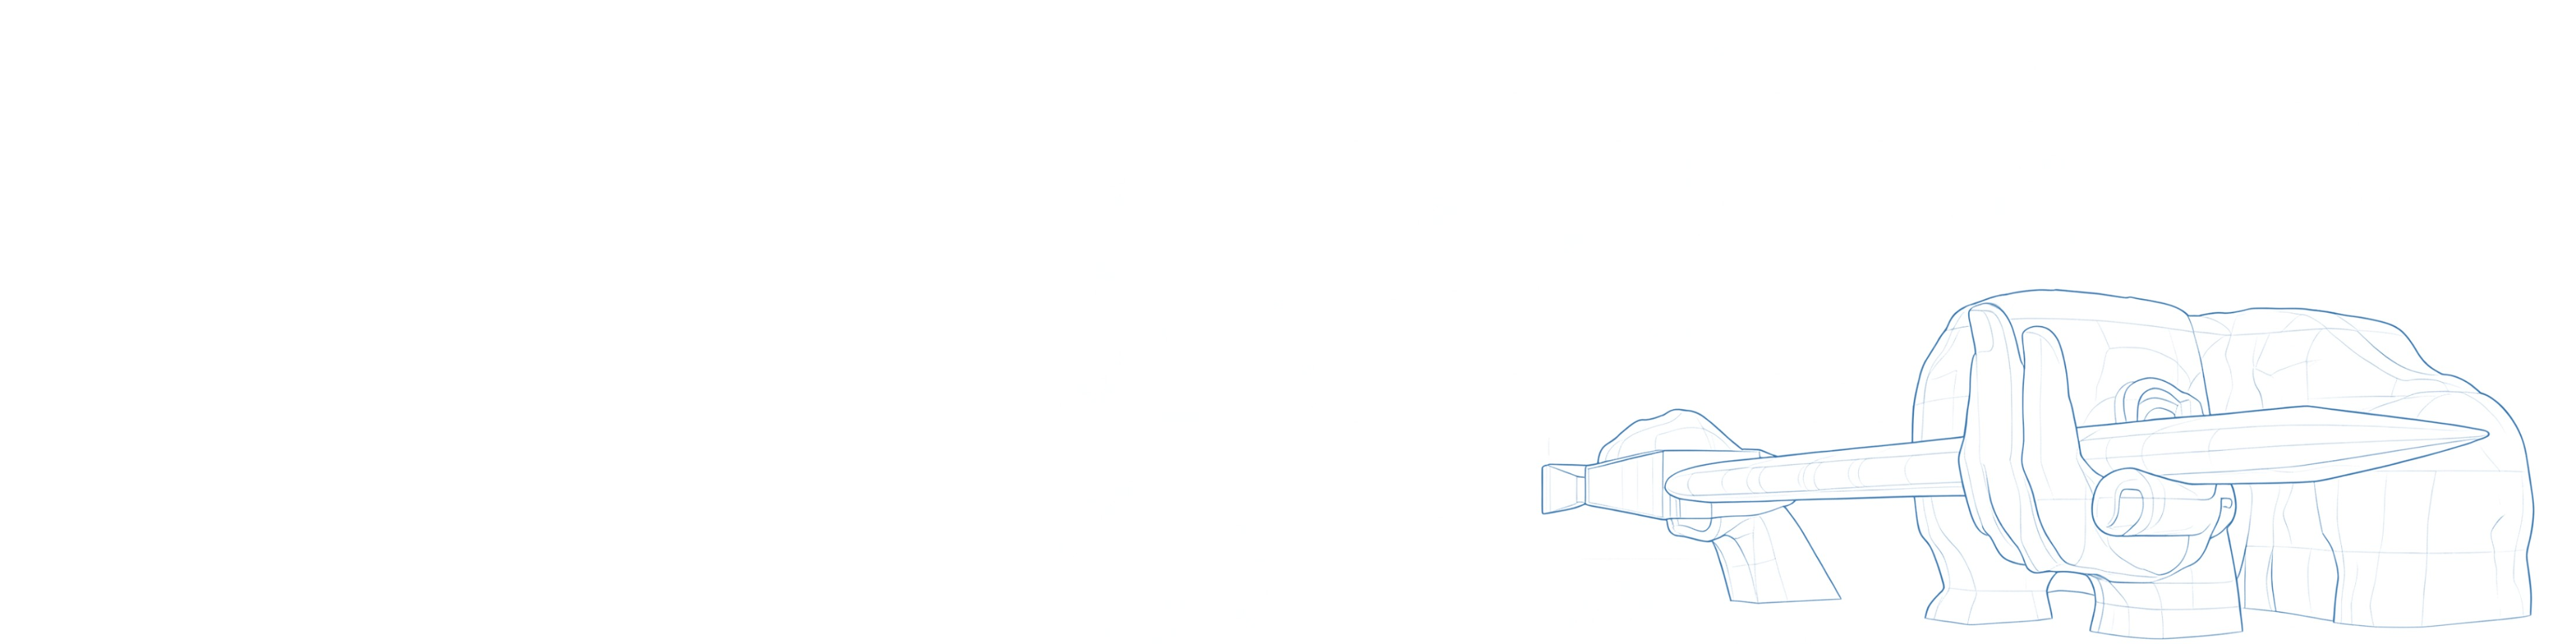
\includegraphics[width=\paperwidth]{src/figure/toc_blue.jpg}};
            \node[anchor=north west, inner sep=0pt]
                at ([yshift=-0.15748\PageHeight, xshift=0.15498\PageHeight]current page.north west)
                {\fontsize{0.06641\PageHeight}{0.07378\PageHeight}\bfseries\color{NPUBlue} 目录};
        \end{tikzpicture}

        \vspace{\dimexpr 1cm - \PageTop\relax}
        {\fontsize{0.04796\PageHeight}{0.04796\PageHeight}\bfseries
            \begin{multicols}{2}
                \noindent\tableofcontents
            \end{multicols}
        }
    \end{frame}
}

% ==============================================
% 十三、章节自动过渡页
% ==============================================
\AtBeginSection[]{
\begingroup
\begin{frame}[noframenumbering,plain]
\begin{tikzpicture}[remember picture,overlay]
    \node[anchor=south, inner sep=0pt]
        at (current page.south)
        {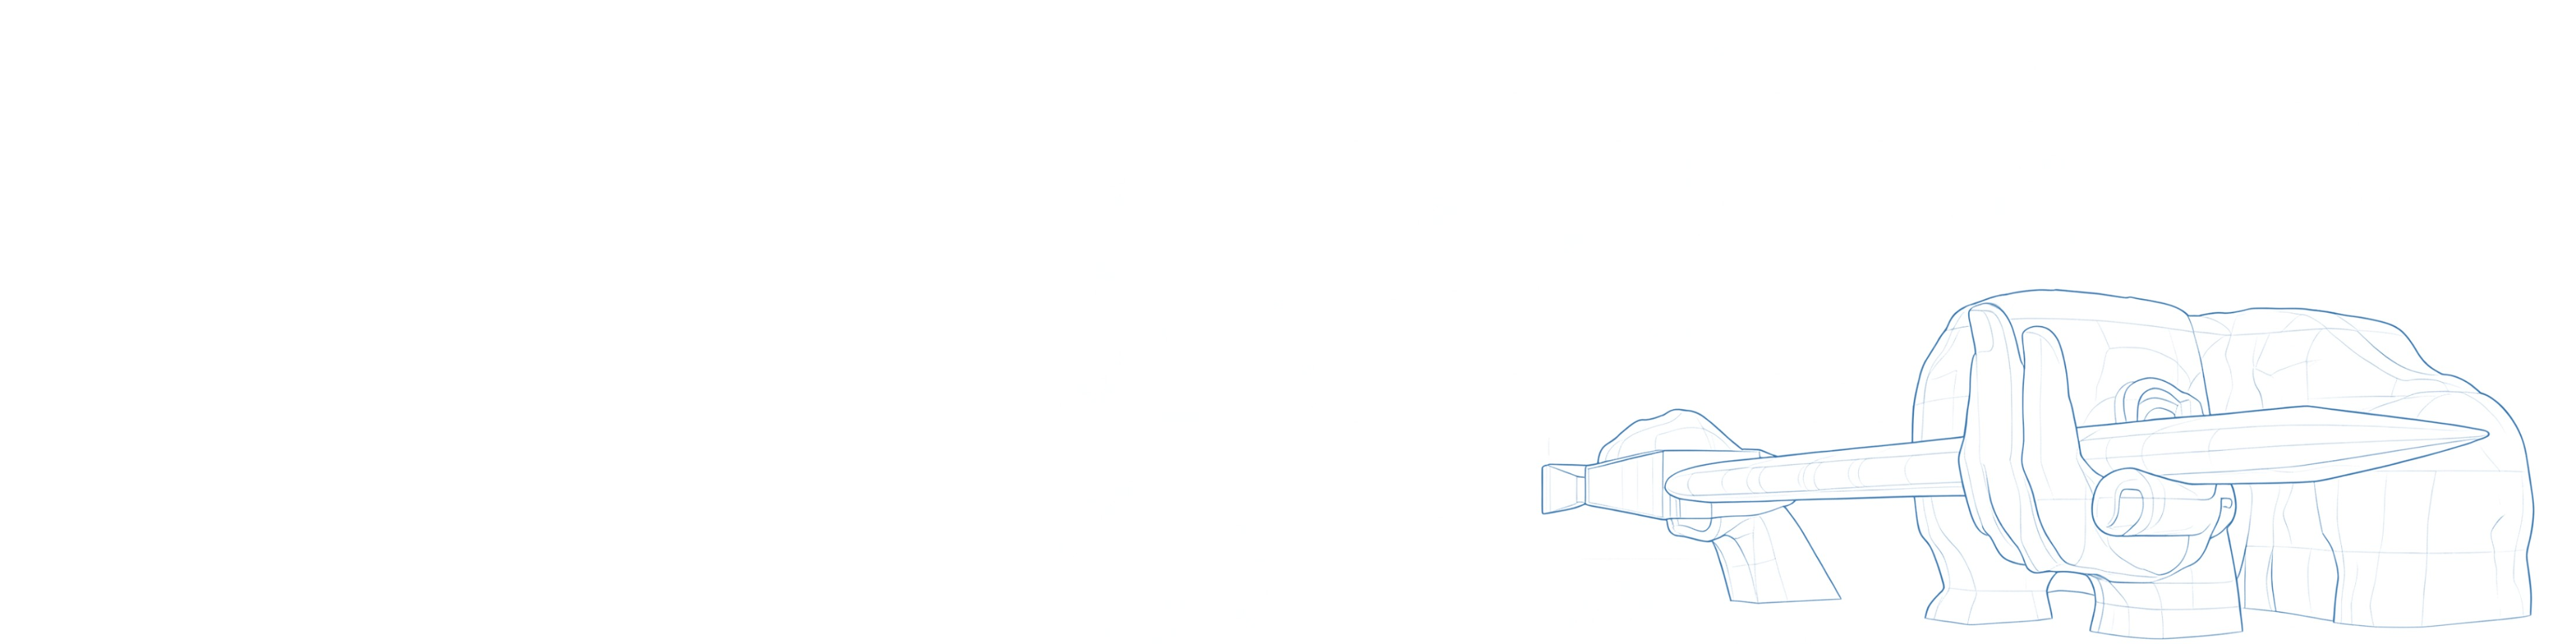
\includegraphics[width=\paperwidth]{src/figure/toc_blue.jpg}};
\end{tikzpicture}

\begin{columns}[c]
% 左侧超大淡数字
\begin{column}{0.25\textwidth}
\centering
\begin{tikzpicture}
\node[
    text=NPUBlue!12, % 淡透明蓝色数字
    font=\bfseries,
    scale=9
]{\thesection};
\end{tikzpicture}
\end{column}

% 右侧标题与标语
\begin{column}{0.55\textwidth}
\raggedleft
% 章节大标题
{\bfseries\LARGE\color{NPUDarkBlue} {\fontsize{38pt}{38pt} \insertsection }} \par
\vspace{3mm}
% 装饰横线
{\color{NPUDarkBlue!70}\rule{0.8\linewidth}{2pt}}\par
\vspace{3mm}
% 底部标语
{\ttfamily\small\color{black!40} 隐姓埋名，为国铸剑}
\end{column}
\end{columns}
\vfill
\end{frame}
\endgroup
}
% ==============================================
% 全局文本变量
% ==============================================
\newcommand{\ReportTitle}{\texttt{NPUBeamer}模板}
\newcommand{\ReportAuthor}{徐爽}
\newcommand{\ReportInstitute}{西北工业大学数学与统计学院}
\newcommand{\ReportTime}{2026年06月14日·西安}


% ===================== 正文开始（综合功能测试） =====================
\begin{document}

% 封面页
\maketitlepage
% 目录页
\mytocpage


\section{字体测试}


\begin{frame}{字体家族}
\begin{table}
\caption{字体家族（Font Family）设置}
\resizebox{0.8\linewidth}{!}{
\begin{tabular}{cccc}
\toprule
     & 无衬线字体   & 衬线字体 & 等宽字体 \\ \midrule
中文     & 思源黑体 &  \textrm{思源宋体} & \texttt{霞鹜文楷}\\ 
英文     & TeX Gyre Heros   & \textrm{TeX Gyre Termes} & \texttt{Source Code Pro}\\  \midrule
中文加粗 & \textbf{思源黑体} &  \textbf{\textrm{思源宋体}} & \textbf{\texttt{霞鹜文楷}}\\ 
英文加粗 & \textbf{TeX Gyre Heros}   & \textbf{\textrm{TeX Gyre Termes}} & \textbf{\texttt{Source Code Pro}}\\  \midrule
中文斜体 & \textit{思源黑体} &  \textit{\textrm{思源宋体}} & \textit{\texttt{霞鹜文楷}}\\ 
英文斜体 & \textit{TeX Gyre Heros}   & \textit{\textrm{TeX Gyre Termes}} & \textit{\texttt{Source Code Pro}}\\  \midrule
中文加粗斜体 & \textbf{\textit{思源黑体}} &  \textbf{\textit{\textrm{思源宋体}}} & \textbf{\textit{\texttt{霞鹜文楷}}}\\ 
英文加粗斜体 & \textbf{\textit{TeX Gyre Heros}}   & \textbf{\textit{\textrm{TeX Gyre Termes}}} & \textbf{\textit{\texttt{Source Code Pro}}}\\
\bottomrule
\end{tabular}
}
\end{table}
\end{frame}

\begin{frame}[fragile]{字体下载}
思源黑体：\url{https://github.com/adobe-fonts/source-han-sans/tree/release#region-specific-subset-otfs}。

\textrm{思源宋体}：\url{https://github.com/adobe-fonts/source-han-serif/tree/release#region-specific-subset-otfs}。

在上面两个页面中点击``China (中国)''进行下载，解压后把所有的\texttt{otf}文件放在\texttt{font}文件夹内。

霞鹜文楷：在页面\url{https://github.com/lxgw/LxgwWenKai/releases}中选择``Source code
(zip)''进行下载，解压后把所有的\texttt{ttf}文件放在\texttt{font}文件夹内。

Source Code Pro：在页面\url{https://github.com/adobe-fonts/source-code-pro/releases/latest}中选择\texttt{otf}对应的压缩包进行下载，解压后把所有的\texttt{otf}文件放在\texttt{font}文件夹内。
\end{frame}

\begin{frame}{普通文本测试}
    该模板的作者为徐爽\footnote{个人主页为\url{https://teacher.nwpu.edu.cn/shuangxu}。}，可以适配日常教学和学术报告场景。本模板的部分设计参考了\texttt{dhuBeamer}\footnote{\url{https://github.com/3000ye/dhuBeamer}。}\texttt{和HiBeamer}\footnote{\url{https://github.com/YLXDXX/hibeamer}。}。

    本模板的默认字号20pt、1.3倍行距。

\end{frame}

\begin{frame}{minipage双栏排版测试}

如果希望minipage首行缩进2个字符，那么需要在环境内先进行设置\texttt{\setlength{\parindent}{2em}}：


\begin{minipage}{0.48\textwidth}
    \setlength{\parindent}{2em}
    这是左栏文字。这是左栏文字。这是左栏文字。
\end{minipage}
\hfill
\begin{minipage}{0.48\textwidth}
    \setlength{\parindent}{2em}
    这是右栏文字。这是右栏文字。这是右栏文字。
\end{minipage}


下面是没有设置的效果：


\begin{minipage}{0.48\textwidth}
    这是左栏文字。这是左栏文字。这是左栏文字。
\end{minipage}
\hfill
\begin{minipage}{0.48\textwidth}
    这是右栏文字。这是右栏文字。这是右栏文字。
\end{minipage}

\end{frame}

\begin{frame}[allowframebreaks]{framebreak测试}
测试文字测试文字测试文字测试文字测试文字测试文字测试文字测试文字测试文字测试文字测试文字测试文字测试文字测试文字测试文字测试文字测试文字测试文字测试文字测试文字测试文字测试文字测试文字测试文字测试文字测试文字测试文字测试文字测试文字测试文字测试文字测试文字测试文字测试文字测试文字测试文字测试文字测试文字测试文字测试文字测试文字测试文字测试文字测试文字测试文字测试文字测试文字测试文字测试文字测试文字测试文字测试文字测试文字测试文字测试文字测试文字测试文字测试文字测试文字测试文字测试文字测试文字测试文字测试文字测试文字测试文字测试文字测试文字测试文字测试文字测试文字测试文字测试文字
\framebreak
测试文字测试文字测试文字测试文字测试文字测试文字测试文字测试文字测试文字测试文字测试文字测试文字测试文字测试文字测试文字测试文字测试文字测试文字测试文字测试文字测试文字测试文字测试文字测试文字测试文字测试文字测试文字测试文字测试文字测试文字测试文字测试文字测试文字测试文字测试文字测试文字测试文字测试文字测试文字测试文字测试文字测试文字测试文字测试文字测试文字测试文字测试文字测试文字测试文字测试文字测试文字测试文字测试文字测试文字测试文字测试文字测试文字测试文字测
\framebreak
试文字测试文字测试文字测试文字测试文字测试文字测试文字测试文字测试文字测试文字测试文字测试文字测试文字测试文字测试文字测试文字测试文字测试文字测试文字测试文字
\end{frame}

% ========== 第二部分：有序列表 + 区块环境 ==========
\section{列表环境}
\begin{frame}{有序列表测试}
    \begin{enumerate}
        \item 有序条目一
        \item 有序条目二
            \begin{enumerate}
                \item 子有序条目1
                \item 子有序条目2
                    \begin{enumerate}
                        \item 孙有序条目1
                        \item 孙有序条目2
                    \end{enumerate}
            \end{enumerate}
    \end{enumerate}
\end{frame}

\begin{frame}{无序列表测试}
    \begin{itemize}
        \item 有序条目一
        \item 有序条目二
            \begin{itemize}
                \item 子有序条目1
                \item 子有序条目2
                    \begin{itemize}
                        \item 孙有序条目1
                        \item 孙有序条目2
                    \end{itemize}
            \end{itemize}
    \end{itemize}
\end{frame}


\section{区块和定理环境}
\begin{frame}
    \frametitle{Block 区块样式测试}
    \begin{block}{标准区块标题}
        这是普通 Block 内容区域，测试区块底色与标题配色。
    \end{block}

    \begin{block}{第二个区块}
        多区块共存测试，验证间距与样式一致性。
    \end{block}

    \begin{exampleblock}{举例区块标题}
        这是 ExampleBlock 内容区域，测试区块底色与标题配色。
    \end{exampleblock}

    \begin{exampleblock}{第二个区块}
        多区块共存测试，验证间距与样式一致性。
    \end{exampleblock}

    \begin{alertblock}{警示区块标题}
        这是 AlertBlock 内容区域，测试区块底色与标题配色。
    \end{alertblock}

    \begin{alertblock}{第二个区块}
        多区块共存测试，验证间距与样式一致性。
    \end{alertblock}
\end{frame}

\begin{frame}[allowframebreaks]{定理环境}
\begin{theorem}[标题]
内容
\end{theorem}
\begin{lemma}[标题]
内容
\end{lemma}
\begin{definition}[标题]
内容
\end{definition}
\begin{corollary}[标题]
内容
\end{corollary}
\begin{proposition}[标题]
内容
\end{proposition}
\begin{remark}[标题]
内容
\end{remark}
\begin{example}[标题]
内容
\end{example}
\begin{exercise}[标题]
内容
\end{exercise}
\end{frame}


% ========== 第三部分：数学公式 ==========
\section{公式}
\begin{frame}[allowframebreaks]{公式环境全测试}
\textbf{1. 行内公式}
实数域满足 $a+b=b+a$，基本不等式 $x^2+y^2 \ge 2xy$。

\vspace{1em}
\textbf{2. 行间无编号公式 \texttt{equation*}}
\begin{equation*}
f(x) = \sin x + \cos x + e^x - \ln x
\end{equation*}

\vspace{1em}
\textbf{3. 单行有编号 \texttt{equation}}
\begin{equation}
\lim_{x\to+\infty} \frac{\sqrt{x^2+1}}{x} = 1
\end{equation}

\vspace{1em}
\textbf{4. 多行对齐 \texttt{align}}
\begin{align}
u_t &= a^2 u_{xx} \\
u(0,t) &= 0 \\
u(x,0) &= \varphi(x)
\end{align}

\vspace{1em}
\textbf{5. 分段函数 \texttt{cases}}
\[
f(x) =
\begin{cases}
x^2, & x\ge 0, \\
-x,  & x<0.
\end{cases}
\]

\vspace{1em}
\textbf{6. 矩阵 / 行列式}
\[
A=
\begin{pmatrix}
1 & 2 & 3 \\
4 & 5 & 6 \\
7 & 8 & 9
\end{pmatrix},\quad
|B|=
\begin{vmatrix}
\alpha & \beta \\
\gamma & \delta
\end{vmatrix}
\]

\vspace{1em}
\textbf{7. 求和、积分、乘积}
\[
\sum_{k=1}^n k = \dfrac{n(n+1)}{2},\quad
\int_0^{+\infty} e^{-x}\,\mathrm{d}x = 1,\quad
\prod_{i=1}^m (1+x_i)
\]

\vspace{1em}
\textbf{8. 集合、逻辑符号}
\[
x\in \mathbb{R},\quad A\subset B,\quad
\forall x,\ \exists y,\quad
p \implies q
\]

\vspace{1em}
\textbf{9. 定理环境内嵌公式}

\begin{theorem}[均值不等式]
设 $a_1,a_2,\dots,a_n>0$，则
\[
\frac{a_1+a_2+\cdots+a_n}{n}
\ge \sqrt[n]{a_1a_2\cdots a_n}.
\]
\end{theorem}

\textbf{10. 公式内中文}

$$x是自变量$$

\end{frame}



% ========== 第四部分：图片与图文布局 ==========
\section{图表测试}
\begin{frame}
    \frametitle{单张图片展示}
    \begin{figure}
    \centering
    
\includegraphics[width=0.5\linewidth]{src/figure/titlepage_cover.jpg}
    \caption{示例图片}
    \end{figure}
\end{frame}

\begin{frame}
    \frametitle{多张图片展示}
    \begin{figure}[htbp]
        \centering
        \begin{minipage}[t]{0.48\textwidth}
            \centering
            
\includegraphics[width=0.5\linewidth]{src/figure/titlepage_cover.jpg}
            \caption{图片1}
        \end{minipage}
        \begin{minipage}[t]{0.48\textwidth}
            \centering
            
\includegraphics[width=0.5\linewidth]{src/figure/titlepage_cover.jpg}
            \caption{图片2}
        \end{minipage}
    \end{figure}
\end{frame}

\begin{frame}
    \frametitle{表格}
    \begin{table}[!ht]
    \centering
    \begin{tabular}{|l|l|l|}
        \hline
        Mercedes & S 450 & 3.0T \\ \hline
        BMW & M760 Li & 4.4T \\ \hline
        Audi & Rs 6 Avant & 4.0T \\ \hline
    \end{tabular}
    \caption{示例表格}
    \end{table}
\end{frame}

\begin{frame}[fragile]{lstlisting环境}

\begin{lstlisting}[language=TeX]
\begin{itemize}
  \item A \item B
  \item C
  \begin{itemize}
    \item C-1
  \end{itemize}
\end{itemize}
\end{lstlisting}

\end{frame}



\begin{frame}{测试算法排版}
  \begin{algorithm}[H]
    \caption{测试算法}
    \begin{algorithmic}[1]
      % 注意：这里使用原生首字母大写的 \Require 和 \Ensure
      \Require 数组 $A$
      \Ensure 排序后的数组 $A$
      \If{$A$ 为空}
        \State \Return $A$
      \EndIf
      \For{$i \gets 1$ 到 $n$}
        \State 处理 $A[i]$
      \EndFor
    \end{algorithmic}
  \end{algorithm}
\end{frame}




\section{逐帧展示}
\begin{frame}{pause测试}
    \begin{itemize} 
        \item 大家都会\LaTeX{}，好多学校都有自己的Beamer主题 \pause
        \item 中文支持请选择 Xe\LaTeX{} 编译选项
    \end{itemize}
\end{frame}

\begin{frame}{href超链接与url网址}

\href{http://far.tooold.cn/post/latex/beamertsinghua}{\color{purple}{链接}}

\url{https://www.latexstudio.net/archives/4051.html}

\end{frame}



\begin{frame}{参考文献测试}
引用\cite{pwrctv_tgrs2024}，引用\cite{balmf2022_tgrs}
\end{frame}


\begin{frame}[allowframebreaks]{参考文献}
\fontsize{0.0369\PageHeight}{0.0369\PageHeight}\selectfont
\bibliographystyle{unsrt}   % 样式
\bibliography{ref}          % bibtex文件
\end{frame}



\end{document}

